% M36: Per-Procedure Accuracy Breakdown — All 6 Policies
% Usage: % M36: Per-Procedure Accuracy Breakdown — All 6 Policies
% Usage: % M36: Per-Procedure Accuracy Breakdown — All 6 Policies
% Usage: % M36: Per-Procedure Accuracy Breakdown — All 6 Policies
% Usage: \input{figures/per_procedure_breakdown.tex} inside a figure environment
% Requires: \usepackage{pgfplots} and \pgfplotsset{compat=1.18}

\definecolor{colCQL}{RGB}{46,204,113}    % green
\definecolor{colIQL}{RGB}{52,152,219}    % blue
\definecolor{colBC}{RGB}{155,89,182}     % purple
\definecolor{colFK3}{RGB}{231,76,60}     % red
\definecolor{colFK5}{RGB}{243,156,18}    % orange
\definecolor{colHeur}{RGB}{26,188,156}   % teal

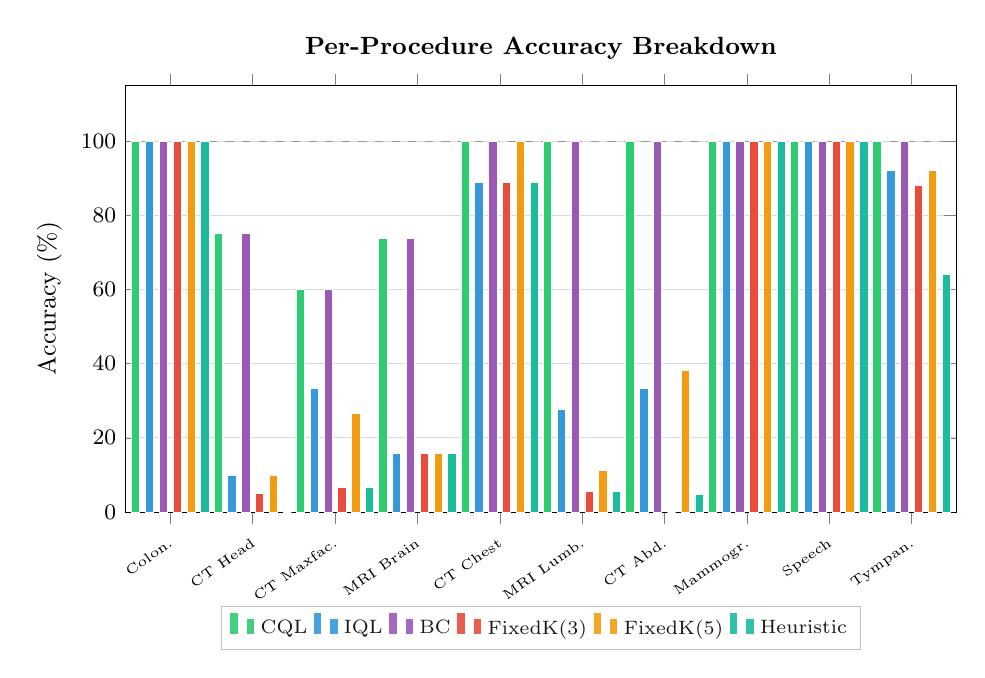
\begin{tikzpicture}
\begin{axis}[
    width=\textwidth,
    height=7cm,
    ybar,
    bar width=3pt,
    enlarge x limits=0.06,
    symbolic x coords={
        {Colon.},
        {CT Head},
        {CT Maxfac.},
        {MRI Brain},
        {CT Chest},
        {MRI Lumb.},
        {CT Abd.},
        {Mammogr.},
        {Speech},
        {Tympan.}
    },
    xtick=data,
    x tick label style={font=\tiny, align=center, rotate=35, anchor=north east},
    ylabel={Accuracy (\%)},
    ylabel style={font=\small},
    ymin=0, ymax=115,
    ymajorgrids=true,
    grid style={gray!30},
    title={\textbf{Per-Procedure Accuracy Breakdown}},
    title style={font=\small},
    tick label style={font=\footnotesize},
    legend style={
        at={(0.5,-0.22)},
        anchor=north,
        legend columns=6,
        font=\scriptsize,
        draw=gray!50,
        fill=white,
        fill opacity=0.9,
    },
    extra y ticks={100},
    extra y tick labels={},
    extra y tick style={grid style={black, dashed, thin, opacity=0.3}},
]

% CQL
\addplot[fill=colCQL, draw=white, line width=0.3pt] coordinates {
    ({Colon.}, 100.0) ({CT Head}, 75.0) ({CT Maxfac.}, 60.0) ({MRI Brain}, 73.7)
    ({CT Chest}, 100.0) ({MRI Lumb.}, 100.0) ({CT Abd.}, 100.0) ({Mammogr.}, 100.0)
    ({Speech}, 100.0) ({Tympan.}, 100.0)
};
\addlegendentry{CQL}

% IQL
\addplot[fill=colIQL, draw=white, line width=0.3pt] coordinates {
    ({Colon.}, 100.0) ({CT Head}, 10.0) ({CT Maxfac.}, 33.3) ({MRI Brain}, 15.8)
    ({CT Chest}, 88.9) ({MRI Lumb.}, 27.8) ({CT Abd.}, 33.3) ({Mammogr.}, 100.0)
    ({Speech}, 100.0) ({Tympan.}, 92.0)
};
\addlegendentry{IQL}

% BC
\addplot[fill=colBC, draw=white, line width=0.3pt] coordinates {
    ({Colon.}, 100.0) ({CT Head}, 75.0) ({CT Maxfac.}, 60.0) ({MRI Brain}, 73.7)
    ({CT Chest}, 100.0) ({MRI Lumb.}, 100.0) ({CT Abd.}, 100.0) ({Mammogr.}, 100.0)
    ({Speech}, 100.0) ({Tympan.}, 100.0)
};
\addlegendentry{BC}

% FixedK(3)
\addplot[fill=colFK3, draw=white, line width=0.3pt] coordinates {
    ({Colon.}, 100.0) ({CT Head}, 5.0) ({CT Maxfac.}, 6.7) ({MRI Brain}, 15.8)
    ({CT Chest}, 88.9) ({MRI Lumb.}, 5.6) ({CT Abd.}, 0.0) ({Mammogr.}, 100.0)
    ({Speech}, 100.0) ({Tympan.}, 88.0)
};
\addlegendentry{FixedK(3)}

% FixedK(5)
\addplot[fill=colFK5, draw=white, line width=0.3pt] coordinates {
    ({Colon.}, 100.0) ({CT Head}, 10.0) ({CT Maxfac.}, 26.7) ({MRI Brain}, 15.8)
    ({CT Chest}, 100.0) ({MRI Lumb.}, 11.1) ({CT Abd.}, 38.1) ({Mammogr.}, 100.0)
    ({Speech}, 100.0) ({Tympan.}, 92.0)
};
\addlegendentry{FixedK(5)}

% Heuristic
\addplot[fill=colHeur, draw=white, line width=0.3pt] coordinates {
    ({Colon.}, 100.0) ({CT Head}, 0.0) ({CT Maxfac.}, 6.7) ({MRI Brain}, 15.8)
    ({CT Chest}, 88.9) ({MRI Lumb.}, 5.6) ({CT Abd.}, 4.8) ({Mammogr.}, 100.0)
    ({Speech}, 100.0) ({Tympan.}, 64.0)
};
\addlegendentry{Heuristic}

\end{axis}
\end{tikzpicture}
 inside a figure environment
% Requires: \usepackage{pgfplots} and \pgfplotsset{compat=1.18}

\definecolor{colCQL}{RGB}{46,204,113}    % green
\definecolor{colIQL}{RGB}{52,152,219}    % blue
\definecolor{colBC}{RGB}{155,89,182}     % purple
\definecolor{colFK3}{RGB}{231,76,60}     % red
\definecolor{colFK5}{RGB}{243,156,18}    % orange
\definecolor{colHeur}{RGB}{26,188,156}   % teal

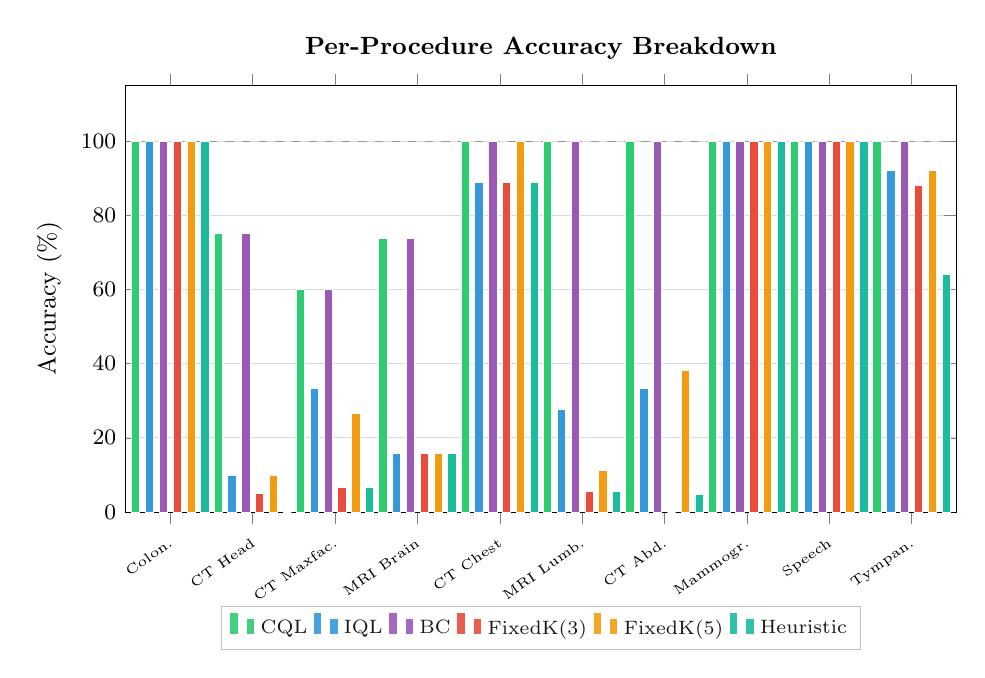
\begin{tikzpicture}
\begin{axis}[
    width=\textwidth,
    height=7cm,
    ybar,
    bar width=3pt,
    enlarge x limits=0.06,
    symbolic x coords={
        {Colon.},
        {CT Head},
        {CT Maxfac.},
        {MRI Brain},
        {CT Chest},
        {MRI Lumb.},
        {CT Abd.},
        {Mammogr.},
        {Speech},
        {Tympan.}
    },
    xtick=data,
    x tick label style={font=\tiny, align=center, rotate=35, anchor=north east},
    ylabel={Accuracy (\%)},
    ylabel style={font=\small},
    ymin=0, ymax=115,
    ymajorgrids=true,
    grid style={gray!30},
    title={\textbf{Per-Procedure Accuracy Breakdown}},
    title style={font=\small},
    tick label style={font=\footnotesize},
    legend style={
        at={(0.5,-0.22)},
        anchor=north,
        legend columns=6,
        font=\scriptsize,
        draw=gray!50,
        fill=white,
        fill opacity=0.9,
    },
    extra y ticks={100},
    extra y tick labels={},
    extra y tick style={grid style={black, dashed, thin, opacity=0.3}},
]

% CQL
\addplot[fill=colCQL, draw=white, line width=0.3pt] coordinates {
    ({Colon.}, 100.0) ({CT Head}, 75.0) ({CT Maxfac.}, 60.0) ({MRI Brain}, 73.7)
    ({CT Chest}, 100.0) ({MRI Lumb.}, 100.0) ({CT Abd.}, 100.0) ({Mammogr.}, 100.0)
    ({Speech}, 100.0) ({Tympan.}, 100.0)
};
\addlegendentry{CQL}

% IQL
\addplot[fill=colIQL, draw=white, line width=0.3pt] coordinates {
    ({Colon.}, 100.0) ({CT Head}, 10.0) ({CT Maxfac.}, 33.3) ({MRI Brain}, 15.8)
    ({CT Chest}, 88.9) ({MRI Lumb.}, 27.8) ({CT Abd.}, 33.3) ({Mammogr.}, 100.0)
    ({Speech}, 100.0) ({Tympan.}, 92.0)
};
\addlegendentry{IQL}

% BC
\addplot[fill=colBC, draw=white, line width=0.3pt] coordinates {
    ({Colon.}, 100.0) ({CT Head}, 75.0) ({CT Maxfac.}, 60.0) ({MRI Brain}, 73.7)
    ({CT Chest}, 100.0) ({MRI Lumb.}, 100.0) ({CT Abd.}, 100.0) ({Mammogr.}, 100.0)
    ({Speech}, 100.0) ({Tympan.}, 100.0)
};
\addlegendentry{BC}

% FixedK(3)
\addplot[fill=colFK3, draw=white, line width=0.3pt] coordinates {
    ({Colon.}, 100.0) ({CT Head}, 5.0) ({CT Maxfac.}, 6.7) ({MRI Brain}, 15.8)
    ({CT Chest}, 88.9) ({MRI Lumb.}, 5.6) ({CT Abd.}, 0.0) ({Mammogr.}, 100.0)
    ({Speech}, 100.0) ({Tympan.}, 88.0)
};
\addlegendentry{FixedK(3)}

% FixedK(5)
\addplot[fill=colFK5, draw=white, line width=0.3pt] coordinates {
    ({Colon.}, 100.0) ({CT Head}, 10.0) ({CT Maxfac.}, 26.7) ({MRI Brain}, 15.8)
    ({CT Chest}, 100.0) ({MRI Lumb.}, 11.1) ({CT Abd.}, 38.1) ({Mammogr.}, 100.0)
    ({Speech}, 100.0) ({Tympan.}, 92.0)
};
\addlegendentry{FixedK(5)}

% Heuristic
\addplot[fill=colHeur, draw=white, line width=0.3pt] coordinates {
    ({Colon.}, 100.0) ({CT Head}, 0.0) ({CT Maxfac.}, 6.7) ({MRI Brain}, 15.8)
    ({CT Chest}, 88.9) ({MRI Lumb.}, 5.6) ({CT Abd.}, 4.8) ({Mammogr.}, 100.0)
    ({Speech}, 100.0) ({Tympan.}, 64.0)
};
\addlegendentry{Heuristic}

\end{axis}
\end{tikzpicture}
 inside a figure environment
% Requires: \usepackage{pgfplots} and \pgfplotsset{compat=1.18}

\definecolor{colCQL}{RGB}{46,204,113}    % green
\definecolor{colIQL}{RGB}{52,152,219}    % blue
\definecolor{colBC}{RGB}{155,89,182}     % purple
\definecolor{colFK3}{RGB}{231,76,60}     % red
\definecolor{colFK5}{RGB}{243,156,18}    % orange
\definecolor{colHeur}{RGB}{26,188,156}   % teal

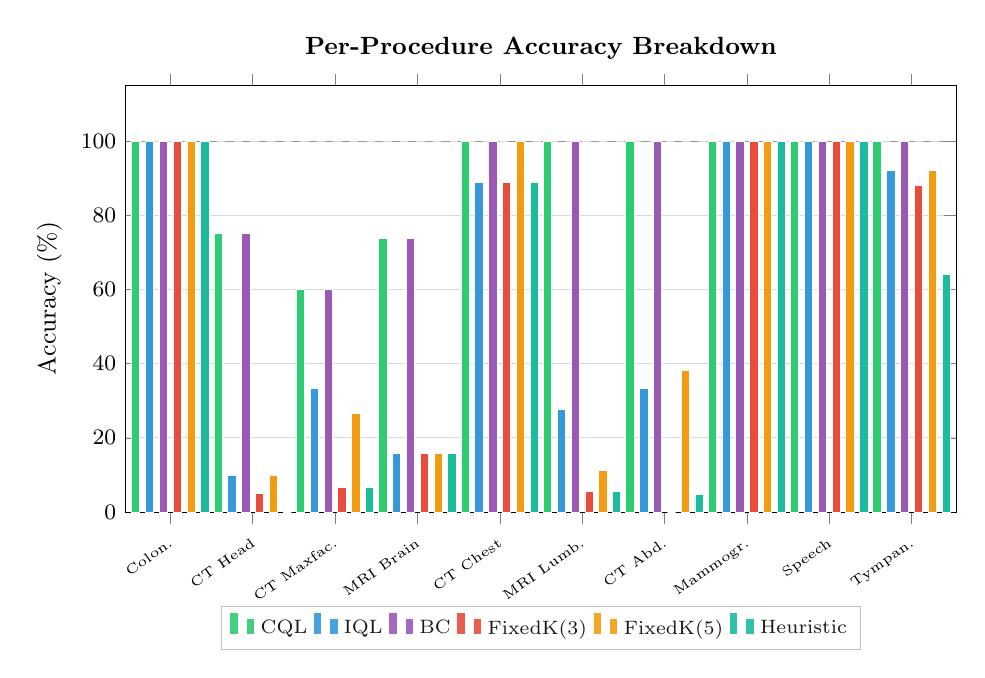
\begin{tikzpicture}
\begin{axis}[
    width=\textwidth,
    height=7cm,
    ybar,
    bar width=3pt,
    enlarge x limits=0.06,
    symbolic x coords={
        {Colon.},
        {CT Head},
        {CT Maxfac.},
        {MRI Brain},
        {CT Chest},
        {MRI Lumb.},
        {CT Abd.},
        {Mammogr.},
        {Speech},
        {Tympan.}
    },
    xtick=data,
    x tick label style={font=\tiny, align=center, rotate=35, anchor=north east},
    ylabel={Accuracy (\%)},
    ylabel style={font=\small},
    ymin=0, ymax=115,
    ymajorgrids=true,
    grid style={gray!30},
    title={\textbf{Per-Procedure Accuracy Breakdown}},
    title style={font=\small},
    tick label style={font=\footnotesize},
    legend style={
        at={(0.5,-0.22)},
        anchor=north,
        legend columns=6,
        font=\scriptsize,
        draw=gray!50,
        fill=white,
        fill opacity=0.9,
    },
    extra y ticks={100},
    extra y tick labels={},
    extra y tick style={grid style={black, dashed, thin, opacity=0.3}},
]

% CQL
\addplot[fill=colCQL, draw=white, line width=0.3pt] coordinates {
    ({Colon.}, 100.0) ({CT Head}, 75.0) ({CT Maxfac.}, 60.0) ({MRI Brain}, 73.7)
    ({CT Chest}, 100.0) ({MRI Lumb.}, 100.0) ({CT Abd.}, 100.0) ({Mammogr.}, 100.0)
    ({Speech}, 100.0) ({Tympan.}, 100.0)
};
\addlegendentry{CQL}

% IQL
\addplot[fill=colIQL, draw=white, line width=0.3pt] coordinates {
    ({Colon.}, 100.0) ({CT Head}, 10.0) ({CT Maxfac.}, 33.3) ({MRI Brain}, 15.8)
    ({CT Chest}, 88.9) ({MRI Lumb.}, 27.8) ({CT Abd.}, 33.3) ({Mammogr.}, 100.0)
    ({Speech}, 100.0) ({Tympan.}, 92.0)
};
\addlegendentry{IQL}

% BC
\addplot[fill=colBC, draw=white, line width=0.3pt] coordinates {
    ({Colon.}, 100.0) ({CT Head}, 75.0) ({CT Maxfac.}, 60.0) ({MRI Brain}, 73.7)
    ({CT Chest}, 100.0) ({MRI Lumb.}, 100.0) ({CT Abd.}, 100.0) ({Mammogr.}, 100.0)
    ({Speech}, 100.0) ({Tympan.}, 100.0)
};
\addlegendentry{BC}

% FixedK(3)
\addplot[fill=colFK3, draw=white, line width=0.3pt] coordinates {
    ({Colon.}, 100.0) ({CT Head}, 5.0) ({CT Maxfac.}, 6.7) ({MRI Brain}, 15.8)
    ({CT Chest}, 88.9) ({MRI Lumb.}, 5.6) ({CT Abd.}, 0.0) ({Mammogr.}, 100.0)
    ({Speech}, 100.0) ({Tympan.}, 88.0)
};
\addlegendentry{FixedK(3)}

% FixedK(5)
\addplot[fill=colFK5, draw=white, line width=0.3pt] coordinates {
    ({Colon.}, 100.0) ({CT Head}, 10.0) ({CT Maxfac.}, 26.7) ({MRI Brain}, 15.8)
    ({CT Chest}, 100.0) ({MRI Lumb.}, 11.1) ({CT Abd.}, 38.1) ({Mammogr.}, 100.0)
    ({Speech}, 100.0) ({Tympan.}, 92.0)
};
\addlegendentry{FixedK(5)}

% Heuristic
\addplot[fill=colHeur, draw=white, line width=0.3pt] coordinates {
    ({Colon.}, 100.0) ({CT Head}, 0.0) ({CT Maxfac.}, 6.7) ({MRI Brain}, 15.8)
    ({CT Chest}, 88.9) ({MRI Lumb.}, 5.6) ({CT Abd.}, 4.8) ({Mammogr.}, 100.0)
    ({Speech}, 100.0) ({Tympan.}, 64.0)
};
\addlegendentry{Heuristic}

\end{axis}
\end{tikzpicture}
 inside a figure environment
% Requires: \usepackage{pgfplots} and \pgfplotsset{compat=1.18}

\definecolor{colCQL}{RGB}{46,204,113}    % green
\definecolor{colIQL}{RGB}{52,152,219}    % blue
\definecolor{colBC}{RGB}{155,89,182}     % purple
\definecolor{colFK3}{RGB}{231,76,60}     % red
\definecolor{colFK5}{RGB}{243,156,18}    % orange
\definecolor{colHeur}{RGB}{26,188,156}   % teal

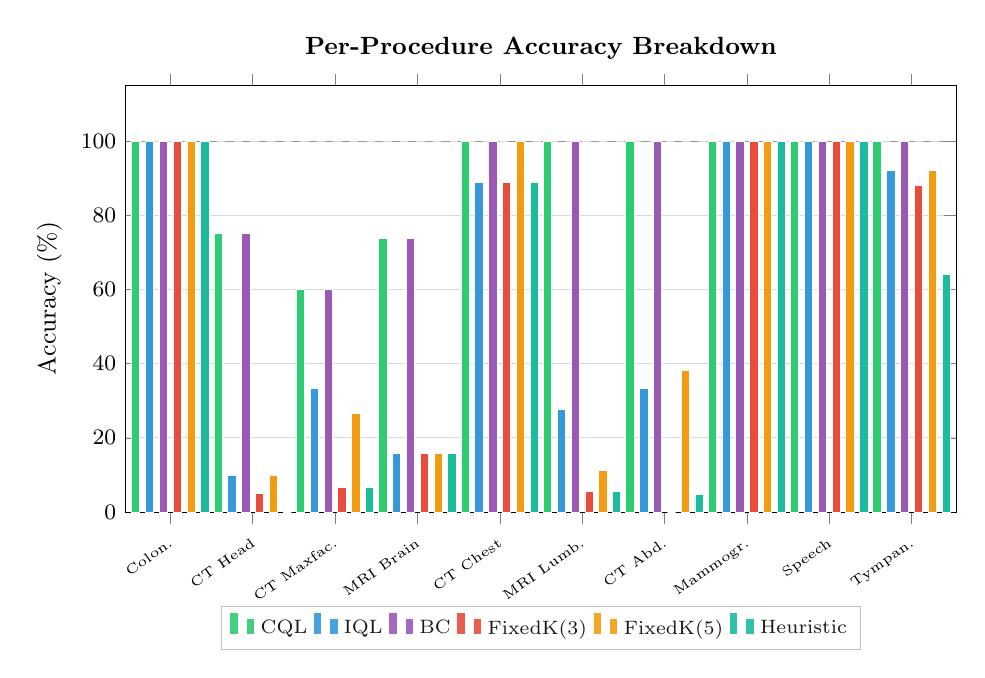
\begin{tikzpicture}
\begin{axis}[
    width=\textwidth,
    height=7cm,
    ybar,
    bar width=3pt,
    enlarge x limits=0.06,
    symbolic x coords={
        {Colon.},
        {CT Head},
        {CT Maxfac.},
        {MRI Brain},
        {CT Chest},
        {MRI Lumb.},
        {CT Abd.},
        {Mammogr.},
        {Speech},
        {Tympan.}
    },
    xtick=data,
    x tick label style={font=\tiny, align=center, rotate=35, anchor=north east},
    ylabel={Accuracy (\%)},
    ylabel style={font=\small},
    ymin=0, ymax=115,
    ymajorgrids=true,
    grid style={gray!30},
    title={\textbf{Per-Procedure Accuracy Breakdown}},
    title style={font=\small},
    tick label style={font=\footnotesize},
    legend style={
        at={(0.5,-0.22)},
        anchor=north,
        legend columns=6,
        font=\scriptsize,
        draw=gray!50,
        fill=white,
        fill opacity=0.9,
    },
    extra y ticks={100},
    extra y tick labels={},
    extra y tick style={grid style={black, dashed, thin, opacity=0.3}},
]

% CQL
\addplot[fill=colCQL, draw=white, line width=0.3pt] coordinates {
    ({Colon.}, 100.0) ({CT Head}, 75.0) ({CT Maxfac.}, 60.0) ({MRI Brain}, 73.7)
    ({CT Chest}, 100.0) ({MRI Lumb.}, 100.0) ({CT Abd.}, 100.0) ({Mammogr.}, 100.0)
    ({Speech}, 100.0) ({Tympan.}, 100.0)
};
\addlegendentry{CQL}

% IQL
\addplot[fill=colIQL, draw=white, line width=0.3pt] coordinates {
    ({Colon.}, 100.0) ({CT Head}, 10.0) ({CT Maxfac.}, 33.3) ({MRI Brain}, 15.8)
    ({CT Chest}, 88.9) ({MRI Lumb.}, 27.8) ({CT Abd.}, 33.3) ({Mammogr.}, 100.0)
    ({Speech}, 100.0) ({Tympan.}, 92.0)
};
\addlegendentry{IQL}

% BC
\addplot[fill=colBC, draw=white, line width=0.3pt] coordinates {
    ({Colon.}, 100.0) ({CT Head}, 75.0) ({CT Maxfac.}, 60.0) ({MRI Brain}, 73.7)
    ({CT Chest}, 100.0) ({MRI Lumb.}, 100.0) ({CT Abd.}, 100.0) ({Mammogr.}, 100.0)
    ({Speech}, 100.0) ({Tympan.}, 100.0)
};
\addlegendentry{BC}

% FixedK(3)
\addplot[fill=colFK3, draw=white, line width=0.3pt] coordinates {
    ({Colon.}, 100.0) ({CT Head}, 5.0) ({CT Maxfac.}, 6.7) ({MRI Brain}, 15.8)
    ({CT Chest}, 88.9) ({MRI Lumb.}, 5.6) ({CT Abd.}, 0.0) ({Mammogr.}, 100.0)
    ({Speech}, 100.0) ({Tympan.}, 88.0)
};
\addlegendentry{FixedK(3)}

% FixedK(5)
\addplot[fill=colFK5, draw=white, line width=0.3pt] coordinates {
    ({Colon.}, 100.0) ({CT Head}, 10.0) ({CT Maxfac.}, 26.7) ({MRI Brain}, 15.8)
    ({CT Chest}, 100.0) ({MRI Lumb.}, 11.1) ({CT Abd.}, 38.1) ({Mammogr.}, 100.0)
    ({Speech}, 100.0) ({Tympan.}, 92.0)
};
\addlegendentry{FixedK(5)}

% Heuristic
\addplot[fill=colHeur, draw=white, line width=0.3pt] coordinates {
    ({Colon.}, 100.0) ({CT Head}, 0.0) ({CT Maxfac.}, 6.7) ({MRI Brain}, 15.8)
    ({CT Chest}, 88.9) ({MRI Lumb.}, 5.6) ({CT Abd.}, 4.8) ({Mammogr.}, 100.0)
    ({Speech}, 100.0) ({Tympan.}, 64.0)
};
\addlegendentry{Heuristic}

\end{axis}
\end{tikzpicture}
